\documentclass[10pt]{article}
\usepackage{url,hyperref}
%\usepackage{times}
\usepackage[left=1in,right=1in,top=1in,bottom=1in]{geometry}
\usepackage[utf8]{inputenc}
\usepackage{amsmath, xparse}
\usepackage{graphicx}
\graphicspath{ {./images/} }

\begin{document}

\noindent \textbf{CAP 6640 -- Natural Language Processing\hspace*{\fill}Spring 2025}\\
\noindent{\bf Homework \#5} \hfill Due date: March 13, 2025

%\vspace*{-0.1in}\paragraph{Instructions:}
%Individual work. Cite all references. All submitted assignments must be typed. Using Latex is required. For \LaTeX, you may use your installation, or online IDEs (no installation required); e.g.,  \href{https://www.overleaf.com/}{www.overleaf.com}. Late submissions by at most 24 hours will be scaled down to 50\%; late beyond 24 hours will be worth 0\%. Total of 40 points. 

\begin{description}
\item[Problem 1:]  \hfill %List and explain four methods for model comparison in natural language processing.

\begin{enumerate}
    \item \textbf{Bag of Vectors:} The Bag of Vectors model represents text as an unordered collection of word embeddings, 
    making it computationally efficient for document classification. While it performs well in tasks that do not require sequential dependencies, 
    its major drawback is the loss of word order and contextual relationships, limiting its effectiveness in complex NLP applications such as machine 
    translation or sentiment analysis. Despite this, performance can be improved by introducing ReLU layers to add non-linearity, 
    but it remains fundamentally constrained by its lack of sequence awareness.
    
    \item \textbf{Window Model:} The Window Model improves upon Bag of Vectors by considering a fixed number of surrounding words, 
    allowing it to capture local context effectively. This makes it particularly useful for single-word classification tasks such as 
    POS tagging and NER. However, since it only considers a small window of words at a time, it struggles with long-range dependencies, 
    making it unsuitable for applications that require a broader contextual understanding.
    
    \item \textbf{CNNs:} CNNs process text by applying convolutional filters over word embeddings, allowing them to detect meaningful 
    n-gram patterns such as sentiment phrases or topic-specific keywords. They excel in text classification tasks in NLP and many others
    as they are highly parallelizable and efficient on GPUs. However, CNNs struggle with long-range dependencies since they primarily 
    focus on local patterns, and they require padding to handle varying sentence lengths, 
    making them less suitable for tasks requiring a strong grasp of word order and context, such as machine translation.
    
    \item \textbf{RNNs:} Unlike CNNs, RNNs are designed to process text sequentially, maintaining a hidden state that carries information from previous words, 
    making them highly effective for tasks like machine translation, speech recognition, and text generation. This structure allows RNNs to model long-term 
    dependencies, providing a more contextual understanding of language. However, they suffer from slow training speeds due to their sequential nature, making 
    them difficult to parallelize. Additionally, they are prone to the vanishing gradient problem, which hinders their ability to capture dependencies over long 
    sequences unless enhancements like LSTMs or GRUs are applied.
\end{enumerate}

\pagebreak

\item[Problem 2:]  \hfill %Differentiate between vertical and horizontal gating.

Gating mechanisms in NNs control the flow of information by selectively allowing or blocking certain values. 
Vertical and horizontal gating are two approaches used to regulate information within deep learning architectures.

\begin{enumerate}
    \item \textbf{Horizontal Gating:} Horizontal gating regulates information flow across time steps in sequential models such as RNNs,
    LSTMs, and GRUs. It helps models retain or discard past information at each time step, making it essential for handling long-term dependencies in sequential data.
    A key example is the forget gate in LSTMs, which determines how much past information should be kept using the formula $f_t = \sigma(W_f h_{t-1} + U_f x_t + b_f)$.
    Horizontal gating is crucial in machine translation, speech recognition, and NLP tasks, where preserving context over time is necessary. 
    However, training these models on very long sequences can be challenging, sometimes requiring attention mechanisms to improve performance.

    \item \textbf{Vertical Gating:} Vertical gating controls information flow across layers in deep neural networks, such as CNNs and ResNets, 
    helping regulate how much information passes from one layer to the next. 
    It is commonly used in Highway Networks and ResNets, where gates determine whether an input is transformed or passed directly to the next layer,
    aiding in gradient flow and feature learning. A key example is the Highway Network, where the transform gate $T(x)$ modulates the proportion of tranformed information
    versus unchanged input using the formula $y = T(x) \cdot H(x) + (1 - T(x)) \cdot x$. Vertical gating is particularly useful in deep architectures to prevent vanishing 
    gradients, making it effective for image classification and other deep learning tasks. However, it does not model temporal dependencies, as it only functions across 
    layers, not time steps.
    
\end{enumerate}

\pagebreak

\item[Problem 3:]  \hfill %Describe how batch normalization improves NLP model performance.

Batch normalization is a widely used technique for CNNs to improve training stability and efficiency.
It works by normalizing activations across a batch, ensuring that NN outputs have zero mean and unit variance, 
which helps to prevent extreme activations that could slow down learning. 
Additionally, batch normalization includes trainable scale $\gamma$ and shift $\beta$  parameters, 
allowing the model to adjust the normalization dynamically rather than simply standardizing all activations.

One of the main advantages of batch normalization is that it reduces internal covariate shift, 
a problem where changing distributions of activations across layers make training less stable. 
By normalizing inputs before they are passed to the next layer, batch normalization ensures that each layer receives consistently scaled data, 
reducing the burden on later layers to adapt to distributional shifts. This leads to faster and more stable training.
Furthermore, it also mitigates vanishing and exploding gradient problems, which commonly occur in deep networks. 
By keeping activations within a reasonable range, it prevents gradients from shrinking too much or growing uncontrollably, 
which can significantly slow down or disrupt training. In addition, it makes parameter initialization less critical, 
since it automatically rescales outputs, reducing the need for carefully chosen weight initializations.
Lastly benefit is that it allows higher learning rates without causing instability, making hyperparameter tuning more forgiving. 
Typically, deep NLP models require very small learning rates to avoid divergence, but batch normalization stabilizes activations, 
enabling the use of more aggressive learning rates that speed up convergence.

\pagebreak

\item[Problem 4:]  \hfill %Explain how very deep CNNs process text.

Traditionally, sequence models like LSTMs and GRUs have dominated NLP due to their ability to handle sequential dependencies. 
However, very deep CNNs which are inspired by image-processing architectures like VGG can be highly effective for NLP, 
particularly in text classification tasks.

Instead of relying on word embeddings and sequential processing, very deep CNNs extract features directly from character-level representations. 
The model consists of multiple stacked convolutional layers, which progressively refine text representations, much like deep CNNs do for images. 
The deeper the network, the more hierarchical and abstract the extracted linguistic features become.

Very deep CNNs apply multiple convolutional layers, followed by pooling layers, to extract patterns in text at various levels. 
This process is similar to how deep CNNs for vision detect simple edges in early layers and complex objects in deeper layers. 
In NLP, this results in low-level character n-grams at shallow layers and high-level semantic representations at deeper layers.
Local pooling at each stage reduces the temporal resolution while retaining key information.
Stacking convolutional layers enables multi-scale text representation, allowing the model to capture both local and long-range dependencies.
This fully convolutional architectures allows for parallel processing, significantly speeding up training.
Deeper CNN architecture improves feature extraction, making the model more effective at capturing linguistic structures.
By leveraging hierarchical feature learning, very deep CNNs can outperform sequence models in text classification tasks, especially when trained on large datasets.

\pagebreak

\item[Problem 5:]  \hfill %Describe how QRNNs work conceptually and mathematically, including their purpose and a supporting figure.

RNNs are effective at capturing sequential dependencies, but they suffer from slow training times due to their sequential nature, 
where each time step depends on the previous one. Quasi-Recurrent Neural Networks, or QRNNs in short, offer a solution by combining the strengths of RNNs and CNNs.
QRNNs use convolutions to capture local dependencies in parallel, similar to CNNs, while gated pooling operations retain long-term dependencies like RNNs.

QRNNs replace the recurrent computations in standard RNNs with 1D convolutions followed by pooling, allowing parallelized sequence processing. 
This is done in two steps. In the first step, QRNNs first apply a 1D convolution over the input sequence to extract features in parallel as

\begin{center}
    $Z_t = $ Conv1D$(X_t, W)$ 
\end{center}

where $X_t$ is the input at time step $t$, $W$ is the convolutional filter, and $Z_t$ is the output feature map. 
Unlike RNNs, which update one state at a time, QRNNs process all time steps simultaneously using convolutional filters. 
As the second step, instead of using a traditional recurrent connection, QRNNs apply a gated pooling mechanism to control the flow of information across time steps as

\begin{center}
    $h_t = f_t \odot h_{t-1} + (1 - f_t) \odot Z_t$
\end{center}

where $f_t$ is the forget gate, $h_{t-1}$ is the previous hidden state, $Z_t$ is the output of the convolutional layer, and $\odot$ denotes element-wise multiplication.
This pooling mechanism mimics the memory function of RNNs, allowing QRNNs to retain sequential information without requiring recurrent operations.

We can illustrate the working process of QRNNs with the following diagram:

\begin{figure}[h]
    \centering
    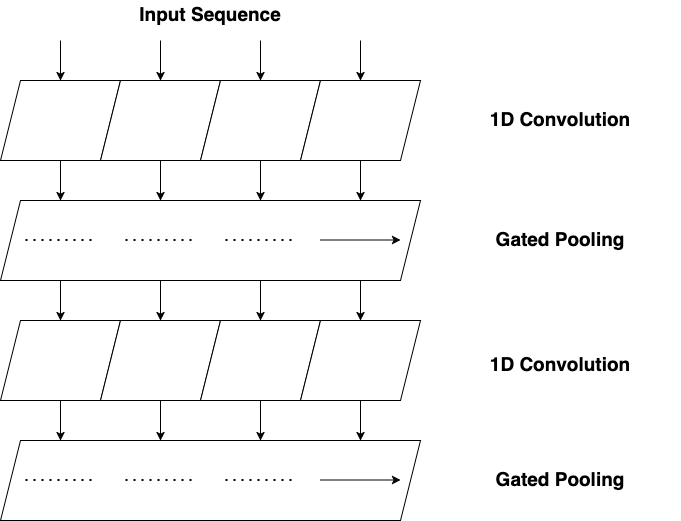
\includegraphics[width=0.48\textwidth]{QRNN_figure.png}
    \caption{Example of a QRNN architecture.}
\end{figure}

This figure higlights the two main components of QRNNs: the convolutional layer for feature extraction and the gated pooling mechanism for sequential processing.

In the convolutions layers, which are named as 1D Convolution in the figure, the input sequence is processed in parallel to extract local features.
Instead of processing tokens one-by-one like RNNs, QRNNs apply convolution filters to extract contextual features from multiple words simultaneously.
This step captures local dependencies, making it significantly faster than RNNs.

The next component after 1D Convolution is named as Gated Pooling in the figure, represent the gated pooling layers, which replace the traditional recurrent mechanism found in RNNs.
Instead of passing hidden states sequentially, gated pooling selectively retains or forgets information across time steps similar to LSTMs.
The dotted lines and rightward arrows indicate that pooling allows long-range dependencies to be retained without explicit recurrence.

Stacking multiple convolution + pooling layers allows QRNNs to capture both short-term and long-term dependencies effectively.

\pagebreak

\item[Problem 6:]  \hfill %Explain the role of subword information in language understanding.

Subword information plays a critical role in NLP by bridging the gap between character-based and word-based representations.
Instead of treating words as singular atomic units, subword models break words into smaller, meaningful components, 
which improves model performance in multiple linguistic and computational aspects.

By incorporating subwords, NLP models can handle rare and previously unseen words, significantly reducing errors in language modeling. 
This approach is particularly valuable for morphologically complex languages like Turkish, where words can take many different forms. 
Additionally, subword modeling helps reduce vocabulary size, making deep learning models more efficient without sacrificing expressiveness.
Another key advantage is its ability to enhance translation quality and tokenization, ensuring better alignment across different languages and writing systems. 
By leveraging subword information, models can achieve better generalization, improved computational efficiency, and enhanced performance in multilingual NLP tasks.

Different languages present unique challenges when processing words, especially those with rich morphology like Turkish. 
In such languages, words are often formed by adding multiple suffixes, which makes subword segmentation essential for better language modeling and machine translation.
In Turkish, a single root word can take on many different forms through suffixation. Consider the word "kitaplarımızdan" (from our books). 
The subword segmentation of this word would be 

\begin{center}
"kitap" + "lar" + "ımız" + "dan"
\end{center}

where each subword represents a meaningful morpheme.

\begin{itemize}
    \item kitap: root word, meaning "book"
    \item lar: plural suffix, books
    \item ımız: possessive suffix, (our books)
    \item dan: ablative case suffix, (from our books) 
\end{itemize}

In a standard word-based model, "kitaplarımızdan" would be treated as a completely separate token, making it hard to generalize across different word forms. 
However, by breaking it down into subwords, an NLP model can recognize morphological structures, improving performance in translation, text generation, and language modeling.

\pagebreak

\item[Problem 7:]  \hfill %Describe fully character-level neural machine translation.

Traditional neural machine translation models rely on word-based tokenization, which can lead to several issues. 
For instance, word-based models struggle with rare or unseen words. They also require large vocabularies to cover all possible words, 
since languages with many word forms like Turkish, Finnish, and Arabic require extensive vocabulary lists.
Lastly, tokenization at the word level may obscure relationships between words with similar roots.

Fully character-level neural machine translation on the other hand is an approach where translation models process text at the character level instead of using 
words or subwords as fundamental units. This method enables models to handle morphologically rich languages, spelling variations, and unknown words, making it 
particularly effective for languages with complex word structures.

Character-level neural machine translation follows the encoder-decoder structure, capturing fine-grained linguistic patterns.
The first step in character-level neural machine translation involves mapping each character in the input sentence to a character embedding.
These embeddings are passed through a CNN, which extract local patterns from the input text.
After extracting character-level features using a CNN, the output is processed through a highway network layer.
The highway network layer acts as a gating mechanism, deciding how much of the original character-level features should be retained or transformed.
This is mathematically formulated as 

\begin{center}
    $t = \sigma(W_T y + b_T)$

    $z = t \odot g(W_H y + b_H) + (1 - t) \odot y$
\end{center}

where $t$ is the transform gate that determines how much new information should be passed forward,
$y$ is the CNN output containing character-level features, $g$ is a non-linear activation function like ReLU,
and $z$ is the refined character-level representation that is sent to higher layers for processing.

The resulting feature representations are then passed to LSTM, which captures long-range dependencies in the sentence.
Finally, the LSTM output is fed into a softmax layer to generate the translation output.

\pagebreak

\item[Problem 8:]  Explain byte pair encoding (BPE).

\pagebreak

\item[Problem 9:]  Compare bottom-up and neural summarization.

\pagebreak

\item[Problem 10:]  Discuss a method for handling irrelevant responses, generic outputs, repetition, and inconsistent persona in natural language generation.


\end{description}

\end{document}